\documentclass[lettersize,journal]{IEEEtran}
\usepackage{amsmath,amsfonts}
\usepackage{algorithmic}
\usepackage{algorithm}
\usepackage{array}
\usepackage[caption=false,font=normalsize,labelfont=sf,textfont=sf]{subfig}
\usepackage{textcomp}
\usepackage{stfloats}
\usepackage{xurl}
\usepackage{verbatim}
\usepackage{graphicx}
\usepackage[table]{xcolor}
\usepackage{multirow}
\usepackage{booktabs}
\newcommand{\good}[1]{\textcolor{green!50!black}{#1}}
\newcommand{\bad}[1]{\textcolor{red!70!black}{#1}}
\newcommand{\TODO}[1]{\textcolor{red!80!black}{\textbf{[TODO: #1]}}}
\usepackage{cite}
\usepackage[colorlinks=true,allcolors=blue,breaklinks=true]{hyperref}
\hyphenation{op-tical net-works semi-conduc-tor IEEE-Xplore}

\begin{document}

\title{A 28\,nm Sparse Transformer Accelerator with \\Row-Wise Run-Length Compression}

\author{Yuan~Liao, Jian Meng, and Jae-sun~Seo \\
School of Electrical and Computer Engineering, Cornell Tech, New York, NY, USA \\
E-mail: \{yl3662, js3528\}@cornell.edu
\thanks{
This work was supported in part by the National Science Foundation under grant 2403723, and the Center for the Co-Design of Cognitive Systems (CoCoSys) under Joint University Microelectronics Program (JUMP) 2.0, a Semiconductor Research Corporation (SRC) program sponsored by Defense Advanced Research Projects Agency (DARPA). (\textit{Corresponding author: Jae-sun Seo})}
\thanks{Yuan Liao, Jian Meng, and Jae-sun Seo are with the School of Electrical and Computer Engineering, Cornell Tech, New York, NY, USA.}}

\markboth{IEEE Transactions on Very Large Scale Integration (VLSI) Systems,~Vol.~XX, No.~XX, XXXX~2026}%
{\TODO{first author} \MakeLowercase{\textit{et al.}}: Sparse Transformer Accelerator with Row-Wise Run-Length Compression}

\maketitle

% =========================================================================
\begin{abstract}
Transformer inference on edge platforms is bounded by four coupled design challenges: scalability across a broad model-size envelope, flexibility across the heterogeneous matrix shapes of attention, projection, and feed-forward kernels, native handling of arbitrary unstructured weight sparsity, and on-die execution of the non-linear operators (softmax, layer normalization, GELU) that dominate latency despite contributing a negligible fraction of FLOPs. This paper presents a 28\,nm sparse transformer accelerator that addresses all four through co-design. A row-wise run-length coding (RRLC) format compresses arbitrary unstructured sparsity into a single-pointer stream that drives a row-wise matrix-multiplication processing element (RMMPE) chain, eliminating zero-weight multiplications without imposing structural constraints. A post-PE pipeline linearizes softmax with a six-entry exponential look-up table and a leading-one-detect logarithm approximation, while a running feature normalization (RFN) scheme folds layer normalization into the existing per-row quantization scale. Silicon characterization of an prototype in TSMC~28\,nm delivers~$1.634$\,TOPS peak performance on a~$90\,\%$-sparse workload and reaches a peak measured energy efficiency of~$20.32$\,TOPS/W on ViT-Base and~$21.93$\,TOPS/W on BERT-base at~$90\,\%$ sparsity. Against prior sparse transformer accelerators under the same sparsity, this chip is $1.62\times$\,--\,$2.47\times$ better in energy efficiency.
\end{abstract}

\begin{IEEEkeywords}
Transformer accelerator, sparse matrix multiplication, run-length coding, row-wise product, softmax linearization, layer normalization.
\end{IEEEkeywords}

% =========================================================================
\section{Introduction}
\label{sec:intro}
\IEEEPARstart{S}{elf-attention}~\cite{Ashish2017attention} has become the workhorse of contemporary vision and language inference. Transformer model families span two orders of magnitude in parameter count and exhibit per-layer dimensions that change layer by layer~\cite{dosovitskiy2021image,Jacob2019bert,kaplan2020scaling}. To support this breadth, a dedicated accelerator must be both highly scalable across the model-size envelope and generic enough to handle the heterogeneous matrix shapes that appear inside a single transformer block. %Throughput is a third axis of pressure. 
In addition, although every block exposes abundant arithmetic parallelism, the attention computation itself serializes through the $Q$, $K$, and $V$ projections before any pairwise score can be evaluated, leaving downstream multiply-and-accumulate (MAC) computation resources idle along the dependency chain. Compounding this, the matrix dimensions of attention, projection, and feed-forward general matrix multiplications (GEMMs) diverge by an order of magnitude, so a rigid 2-D systolic array tile sized for the largest GEMM remains under-utilized on the smaller ones~\cite{Kung1982Systolic}.

\begin{figure}[!t]
    \centering
    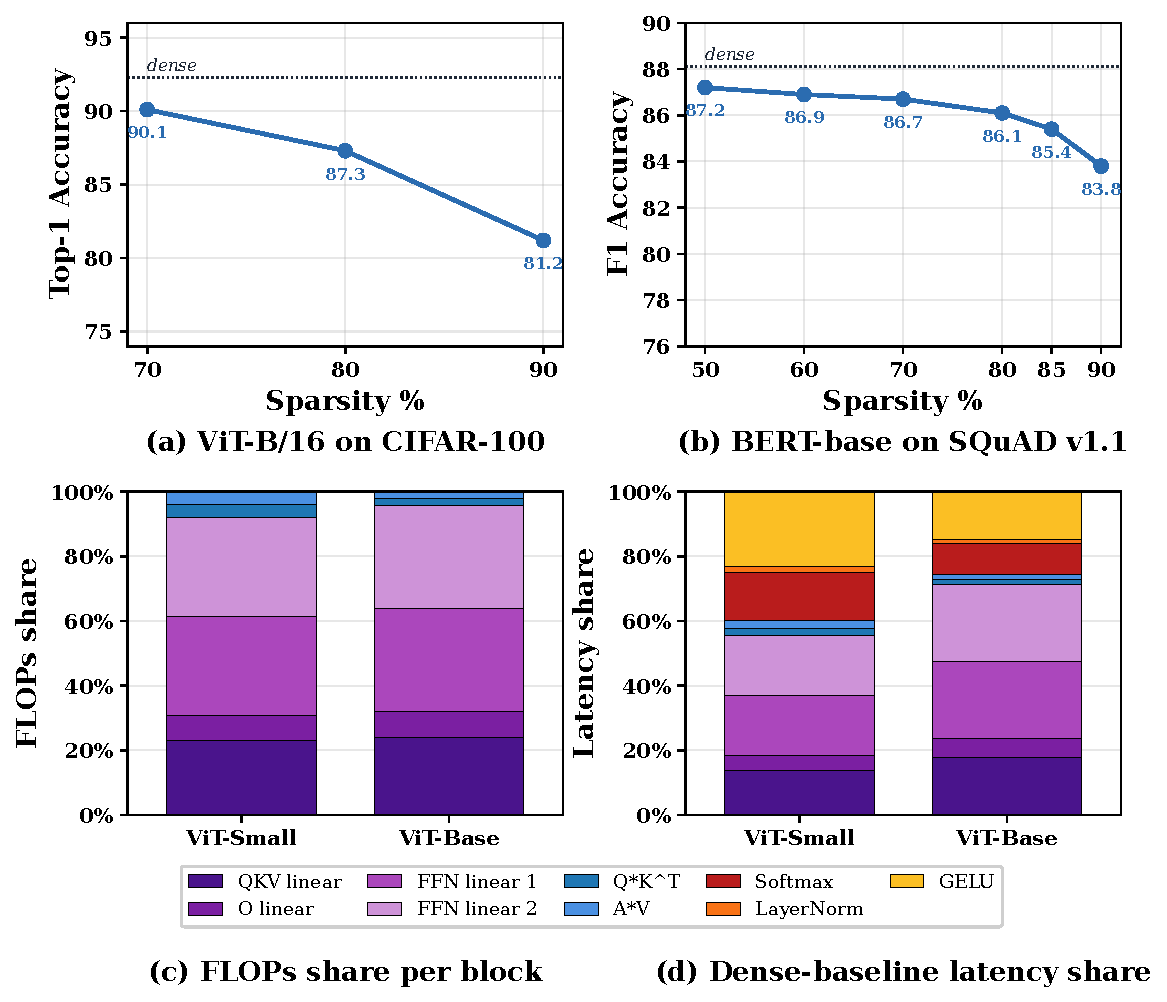
\includegraphics[width=\columnwidth]{figures_analysis/model_profile.pdf}
    \caption{(a, b) ViT-Base and BERT-base accuracy versus unstructured-weight sparsity under PLATON pruning~\cite{zhang2022platon}; dashed lines mark the dense baseline. (c, d) Per-operator share of FLOPs and dense-baseline cycles in one transformer block.}
    \label{fig:profile}
\end{figure}

The established algorithm-side lever for taming this growth is post-training compression. Element-wise pruning preserves transformer accuracy at high sparsity provided the pruning rule scores weights by sensitivity-plus-uncertainty rather than magnitude alone~\cite{zhang2022platon,liu2021sparse,Kyungmin2021sparsevit}. Fig.~\ref{fig:profile}(a) and Fig.~\ref{fig:profile}(b) reproduce the sparsity--accuracy curves of PLATON~\cite{zhang2022platon} for ViT-Base on CIFAR-100 and BERT-base on SQuAD v1.1, respectively. At $80\%$ sparsity, the pruned models maintain %stay within $5$\,--\,$2$\,pp 
2-5\% accuracy degradation, compared to the dense baseline. 
%The hardware story is less tidy. 
On the other hand, the implications for hardware are much less favorable.
Unstructured sparsity fares well on the accuracy precisely because the pruning step has unrestricted freedom over which weights to remove, but that same freedom yields irregular addressing and unaligned MAC operands that penalize rigidly tiled hardware fabrics. Compounding this, the sequence of transpose of~$K$, softmax over~$QK^{\top}$, residual add, and layer normalization couples on-chip operand reuse to the transformer's specific dataflow, and a fixed datapath that handles one stage well typically handles another poorly.

The non-linear operations on the residual path raise a related but distinct concern. Softmax, layer normalization, and the activation function appear inexpensive by FLOPs accounting (Fig.~\ref{fig:profile}(c) attributes under~$0.1\%$ of per-block arithmetic to them), yet Fig.~\ref{fig:profile}(d) shows that the same operators consume $26\%$\,--\,$40\%$ of per-block cycles on a $16{\times}16$ systolic array coupled with $16$ parallel special function units. The cost lies in the exp, square-root, and tanh primitives that anchor these operators: each need to be evaluated iteratively on a precise function unit~\cite{Volder1959CORDIC}. According, na\"ive on-chip implementations either are expensive (precise iterative function units) or degrades accuracy (heavy approximations), so the relevant design question is how to keep the operators on chip without paying either cost.

Taken together, these forces distill the practical bottlenecks of transformer-targeted hardware into four design challenges:
\begin{enumerate}
    \item \textbf{Scalability}: a compute-unit organization whose size is re-targetable across the broad model-size spectrum without datapath redesign.
    \item \textbf{Flexibility}: a single data layout and dataflow that handles the heterogeneous matrix shapes encountered in attention, projection, and feed-forward kernels.
    \item \textbf{Sparsity-compatibility}: native support for arbitrary element-wise sparsity, realized as in-loop skipping of zero MACs.
    \item \textbf{Non-linearity}: an on-chip approximation of softmax and layer normalization that preserves model accuracy while spending less power, area, and latency cost.
\end{enumerate}

Existing transformer accelerators meet these challenges only in part. The approximate-computing processor of~\cite{Yang2022isscc} and the early-exit processor of~\cite{Thierry2023isscc} both support unstructured sparsity and on-chip non-linear functions, but reach their headline efficiency only at a particular operating point: \cite{Yang2022isscc} relies on approximate-computing speculation that assumes simultaneous input and weight sparsity, and \cite{Thierry2023isscc} couples entropy-based early exit, so neither figure reflects a model average across the heterogeneous GEMMs (\textbf{Challenges 1, 2}). \cite{Li2025SparseTrim} provides no on-chip non-linear function unit (\textbf{Challenge 4}), so softmax and layer normalization fall back to off-chip arithmetic and a full transformer cannot execute end-to-end. \cite{Fan2025MultiTaskTransformer} restricts sparsity to a block-wise structured pattern (\textbf{Challenge 3}), which constrains the pruning mask and therefore caps the attainable sparsity and accuracy relative to an unstructured scheme. No prior design satisfies all four challenges on a single fabric.

To attack all four challenges within a single fabric, this paper presents a sparse transformer accelerator built around two co-designed compute primitives. The first is a row-wise matrix multiplication processing element (RMMPE) that executes every GEMM in the transformer in row-wise product form. Because the row-wise schedule is constrained by only one dimension of GEMMs, the same RMMPE handles the attention batched matrix multiplications (BMMs), projection layers, and feed-forward network (FFN) GEMMs with improved utilization compared to 2D architecture (\textbf{Challenges 1 and 2}). RMMPE further consumes inputs and weights in a row-wise run-length coding (RRLC) format, an extension of run-length coding to multi-row groups, that exposes arbitrary unstructured sparsity to the parallel MAC array (\textbf{Challenge 3}). The second primitive is a post-PE processor (PPE) that linearizes softmax through a six-entry exponential look-up and a leading-one-detect logarithm, and folds layer normalization into the per-row quantization scale of a precomputed running feature statistic (\textbf{Challenge 4}).

This article extends our previous conference paper~\cite{Liao2024SparseTransformer} with deeper design choice analysis and replaces the simulation result by the silicon experiment result. The remainder is organized as follows: Section~\ref{sec:algo} develops the algorithm/hardware co-design, Section~\ref{sec:arch} details the accelerator architecture, Section~\ref{sec:results} reports the silicon-measured results and cross-model benchmarks, and Section~\ref{sec:conclusion} concludes the paper.

% =========================================================================


\begin{figure}[!t]
    \centering
    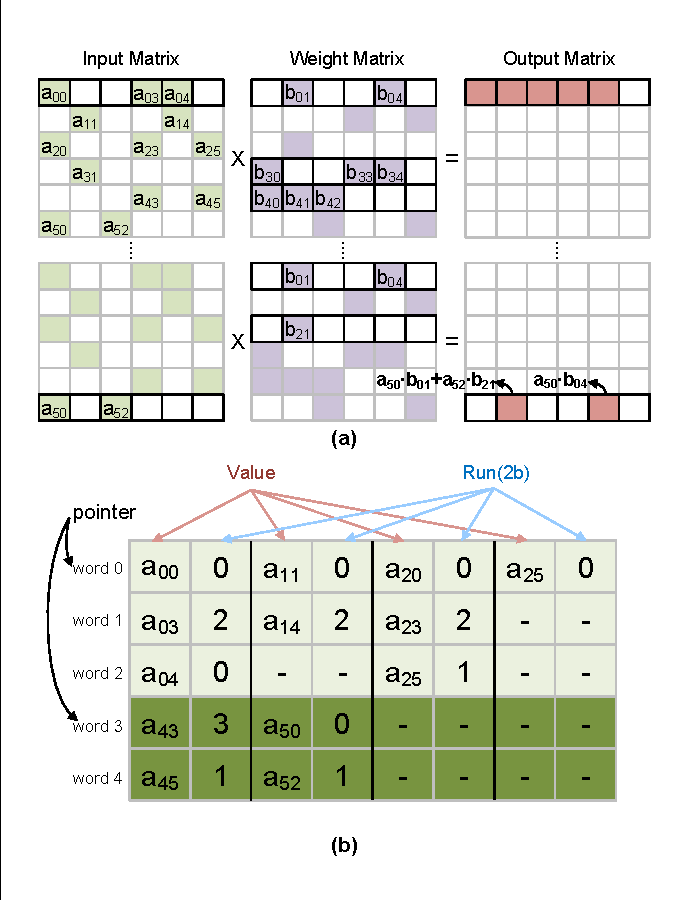
\includegraphics[width=\columnwidth,page=1,trim=1 1 1 1,clip]{figures/TVLSI_drawing.pdf}
    \vspace{-30pt}
    \caption{(a) Row-wise product matrix multiplication and (b) the row-wise run-length coding (RRLC) format applying to the Input Matrix in (a).}
    \label{fig:rwp-rrlc}
\end{figure}

\section{Algorithm and Hardware Co-Design}
\label{sec:algo}

Many sparse transformer accelerators~\cite{Ham2020A3,Liqiang2021Sanger,Hanrui2021SpAtten,Guan2022SALO,Sangyeob2024CTransformer,Sangyeob2025SlimLlama} that concentrate on accelerating only the attention layers by removing the redundant inter-token computations %therefore 
leave the layer normalization layers and, more importantly, the FFN GEMMs untouched. The FFN GEMMs dominate the parameter count in the deeper vision transformers (ViT) and language variants, and the highly specialized attention-only datapath cannot well adapt to executing them, especially since weight sparsity is excessively more prominent than input sparisty in FFN layers. A second issue, common to attention-only and full-transformer accelerators that adopt inner-product schedules, is that layer normalization and the activation function operate row-wise on the output matrix, while inner-product GEMM produces either the entire output at once or a partial output matrix consisting of multiple rows, a mismatch that forces a large output buffer to hold the intermediate results. We address both problems by executing every GEMM in row-wise product form, also known as Gustavson's algorithm~\cite{gustavson1978}.

\subsection{Row-Wise Product Matrix Multiplication}
\label{sec:algo-rwp}

Row-wise product computes one output one at a time by accumulating scaled rows of the weight matrix:
\begin{equation}
    \mathrm{Out}[i,:] = \sum_{j=0}^{K-1} \mathrm{In}[i,j]\cdot \mathrm{Wgt}[j,:].
\label{eq:rwp}
\end{equation}
Fig.~\ref{fig:rwp-rrlc}(a) illustrates the schedule on a small example: each non-zero input element $\mathrm{In}[i,k]$ broadcasts against weight row $k$ to contribute a partial-product row into $\mathrm{Out}[i,:]$, while zero input elements skip their weight-row reads entirely. Four properties of Eq.~\eqref{eq:rwp} make it directly attractive for sparse transformer inference~\cite{Nitish2020MatRaptor}. First, the input, weight, and output tensors all traverse the memory row-wise, allowing a single data format to serve every operand. Second, zero entries of $\mathrm{In}[i,j]$ contribute nothing to the accumulation, so a sparsity-aware scheduler can skip them at zero cycle cost. Third, multiple output rows can be produced concurrently by dispatching independent input rows to parallel MAC arrays. Fourth, only a small number of output rows, rather than the full output matrix, needs to be buffered on chip, removing the large-buffer constraint of inner-product schedules. Together, these four properties address \textbf{Challenges~2} and \textbf{3}: a single dataflow handles every matrix shape, and the zero-skipping is native rather than retroactively fitted.

Prior row-wise-product accelerators~\cite{Nitish2020MatRaptor} suffer from a complementary limitation, however: by computing one output row per multiplier, they leave throughput on the table and do not scale. The familiar sparse-matrix encodings such as compressed sparse column (CSC), coordinate list (COO), and ordinary run-length coding (RLC)) also serialize inherently %naturally 
and resist parallel consumption. We resolve this with the row-wise run-length coding (RRLC) format, which trades a small amount of compressed-stream padding for the ability to feed a $N$-wide multiplier array per cycle. The padding cost is empirically small for the sparsity regimes considered here, and the corresponding throughput gain restores scalability (\textbf{Challenge~1}). The row-wise output further aligns naturally with the row-wise nature of layer normalization and softmax (\textbf{Challenge~4}).

\subsection{Row-Wise Run-Length Coding (RRLC)}
\label{sec:algo-rrlc}

RRLC (Fig.~\ref{fig:rwp-rrlc}(b)) is a multi-row variant of run-length coding. The matrix is partitioned into groups of $N$ contiguous rows ($N{=}8$ in the prototype, matching the row parallelism of one PE), and each group is serialized into a single memory word that concatenates the $N$ rows column by column. Every non-zero element contributes a (\textit{Value},~\textit{Run}) tuple: \textit{Value} carries the 8-bit weight, and the 3-bit \textit{Run} records how many consecutive zeros preceded it. When more than $2^{3}{-}1{=}7$ zeros separate two non-zeros, a placeholder \textit{Value}\,$=0$ tuple is inserted so that the run never overflows. Within a group, rows of differing density are padded with the same placeholder so that all rows in the same group exhausts at the same time. A pointer memory stores the end address of every group, serving two roles: it signals the decoder to stop streaming the current group's tuples, and, because group $g{+}1$ begins immediately after group $g$, it also acts as an index that lets the decoder jump directly to any output row group.

\begin{figure}[!t]
    \centering
    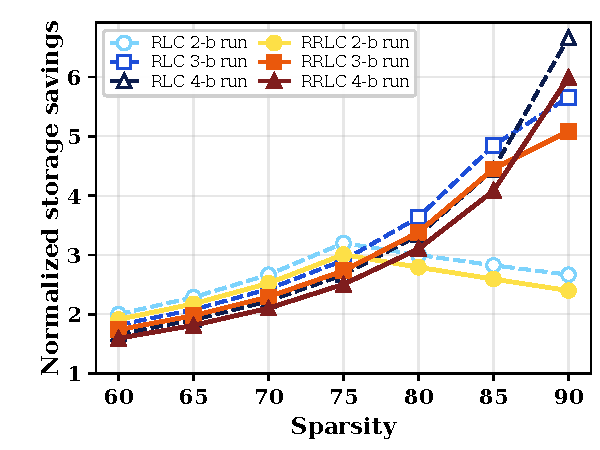
\includegraphics[width=\columnwidth]{figures_analysis/rrlc_storage.pdf}
    \caption{Normalized weight-storage savings versus sparsity for ViT-Base under RLC (dashed) and RRLC (solid, this work) at $R\in\{2,3,4\}$-bit \textit{Run}-field widths.}
    \label{fig:rrlc-storage}
\end{figure}

The choice of three \textit{Run} bits is the empirical optimum for the $75\%$\,--\,$90\%$ sparsity regime targeted by sensitivity-aware pruning of both language and vision transformers. Fig.~\ref{fig:rrlc-storage} quantifies the trade-off on ViT-Base: $R{=}3$ RRLC achieves $2.7\times$, $3.4\times$, $4.5\times$, and $5.1\times$ savings at $75\%$, $80\%$, $85\%$, and $90\%$ sparsity, respectively. $R{=}2$ peaks at $75\%$ sparsity and then plateaus around $2.5\times$ as the $3$-state \textit{Run} field underflows the average run length. $R{=}4$ extends the linear regime further out but pays a per-tuple overhead at every sparsity below $\sim$88$\%$, only surpassing $R{=}3$ at $90\%$ sparsity. The dashed RLC curves are the row-by-row encoding upper bound; RRLC pays a small inter-row-alignment premium ($\sim 5\%$ at $70\%$ sparsity, growing to $\sim$11$\%$ at $90\%$) for the privilege of decoding $N$ rows on a parallel multiplier array. RRLC encoding is performed once per model with the sparse weight offline, and its cost is therefore amortized away from inference. The decoder, detailed in Section~\ref{sec:arch-rmmpe}, consumes the \textit{Run} stream to drive accumulator addresses; the multiplier array thus sees only non-zero weights even though it executes a dense schedule on \textit{Value}.

\subsection{Hardware-Aware Algorithm Design}
\label{sec:algo-hwawer}

Alongside the hardware design, we adopt a small set of algorithm-side choices that make sparsified, INT8 transformer inference viable on the same datapath that performs sparse MAC.

\subsubsection{Model Sparsification}
\label{sec:algo-prune}

Weights are pruned by magnitude with a sparsity ratio that is gradually ramped during training, following the gradient-based ``prune-and-regrow'' procedure of~\cite{liu2021sparse}. Vision transformers tolerate up to $90\%$ element-wise sparsity under this recipe, outperforming the PLATON method of Fig.~\ref{fig:profile}. The sparsity--accuracy trade-off is reported in Section~\ref{sec:results}. The resulting weight masks are unstructured, which is precisely the regime RRLC absorbs.

\subsubsection{Running Feature Normalization (RFN)}
\label{sec:algo-rfn}

Layer normalization~\cite{ba2016layernorm} acts on each token independently. Given an activation tensor $\mathcal{X}\in\mathbb{R}^{B\times N\times F}$ with $B$ samples, $N$ tokens, and $F$ features, the operator computes its statistics $(\mu, \sigma)$ by reducing the $F$-dimensional feature vector \emph{once per token}:
\begin{equation}
    \mathrm{LN}(x_{i})=\gamma\,(x_{i}-\mu)/\sigma+\beta
    \label{eq:ln}
\end{equation}
This is hardware-inefficient on two aspects. First, the per-token reduction across $F$ is serial and data-dependent, so every token stalls the downstream pipeline until its statistics arrive. Second, the resulting scale is dynamic, since a fresh $(\mu, \sigma)$ pair is produced for every token, and therefore cannot be folded into a fixed-point quantizer at calibration time. Substituting batch normalization~\cite{Ioffe2015BatchNorm} does not rescue either issue, because the reduction axes, $B\times N$, do not align with layer normalization's $F$.

The proposed RFN preserves the form of Eq.~\eqref{eq:ln} but moves the reduction off the inference path. During training, $(\mu, \sigma)$ are collected over the $[B, N]$ batch-token plane, leaving one statistic per feature (shape $F$), and tracked as running estimates with momentum $\alpha$:
\begin{align}
    \mu_{r} &= \alpha\,\mu + (1-\alpha)\,\mu_{r}, \\
    \sigma_{r} &= \alpha\,\sigma + (1-\alpha)\,\sigma_{r}.
\end{align}
The training forward pass still normalizes with the instantaneous $(\mu, \sigma)$, so the LN gradient signal that vision transformers rely on is preserved; the running estimates $(\mu_{r}, \sigma_{r})$ are used only at inference. Once training finishes, $(\mu_{r}, \sigma_{r})$ are frozen, and Eq.~\eqref{eq:ln} collapses into a \emph{static} per-feature affine transform of $x_{i}$ with no remaining online reduction. Its scale and bias fold at calibration into the per-row INT8 quantization scale already carried by every PE row, so %on chip 
on-chip computation of an LN-type layer 
reduces to a per-row scale broadcast over the existing quantization-scale bus, without the need of a dedicated normalization datapath, an iterative function unit, or a normalization buffer.


\begin{table}[!t]
    \vspace{10pt}
    \caption{Hardware-aware ViT accuracy on ImageNet-1K (top-1, \%).}
    \label{tab:accuracy}
    \centering
    \footnotesize
    \setlength{\tabcolsep}{3pt}
    \begin{tabular*}{\columnwidth}{@{}l@{\extracolsep{\fill}}cccc@{}}
        \toprule
        Model & FP32 & W/A & SW Acc. & HW Acc. \\
        \midrule
        ViT-Tiny  & 74.34 & 8/8 & 73.04 & 72.02 \\
        ViT-Small & 80.37 & 8/8 & 80.05 & 79.45 \\
        ViT-Base  & 84.54 & 8/8 & 84.52 & 83.88 \\
        \bottomrule
    \end{tabular*}
\end{table}


\subsubsection{Token-Wise Quantization}
\label{sec:algo-quant}

Activations are quantized to INT8 precision with a per-token (per-row) scale factor that shares the per-row quantization-scale bus with RFN; weights use a per-tensor INT8 scale because their distribution is stationary at inference. The per-token granularity preserves the dynamic range of attention scores at sequence lengths where per-tensor quantization saturates~\cite{AWQ,smoothquant}.

\subsubsection{ReLU in Place of GELU}
\label{sec:algo-relu}

The chip implements ReLU rather than GELU~\cite{hendrycks2023GELU} as the FFN activation function. ReLU is a single MSB check on the input and essentially costs no extra cycles or area. GELU, by contrast, would require an additional iterative function unit for its tanh primitive. Fig.~\ref{fig:profile}(d) highlights the cost of executing the original GELU, between $15\%$ and $23\%$ of per-block cycles on its own, and the ReLU substitution eliminates that segment entirely.

\subsubsection{Approximated Softmax}
\label{sec:algo-softmax}

The exact softmax, $y_{i}=\exp(x_{i}-x_{\max})/\sum_{j}\exp(x_{j}-x_{\max})$, couples a per-row maximum, an element-wise exponential, and a reciprocal, all of which are expensive on dedicated functional. Following~\cite{meiqi2018softmax}, the inner exponential is restricted to its 8-bit effective range and tabulated in a six-entry look-up, and the reciprocal is folded into a log-sum-exp pass that reuses the same look-up together with a leading-one-detect logarithm. The on-chip pipeline is detailed in Section~\ref{sec:arch-ppe-softmax}. Combined with RFN-fused LN and the ReLU substitution, the three reformulations collapse the $26\%$\,--\,$40\%$ non-linear latency share of Fig.~\ref{fig:profile}(d) into a small fraction of per-block cycles without requiring any iterative function unit.

Table~\ref{tab:accuracy} reports the cumulative accuracy of the hardware-aware models on ImageNet-1K. The \textbf{SW Acc.} column applies the algorithm-side reformulations of this subsection (INT8 weight/activation quantization, RFN-fused LN, and ReLU in place of GELU) on top of the FP32 baseline. The \textbf{HW Acc.} column additionally accounts for the on-chip softmax LUT approximation. All three ViT scales remain within roughly one percentage point of FP32.


\section{Accelerator Architecture}
\label{sec:arch}

\begin{figure}[!t]
    \centering
    \includegraphics[width=\columnwidth,page=2,trim=20 1 30 1,clip]{figures/TVLSI_drawing.pdf}
    \vspace{-35pt}
    \caption{Overall accelerator architecture. The prototype has the configuration of $N{=}M{=}P{=}8$.}
    \vspace{-10pt}
    \label{fig:arch}
\end{figure}

Fig.~\ref{fig:arch} shows the overall accelerator architecture. The micro-architecture of one RMMPE is detailed in Fig.~\ref{fig:rmmpe}. The chip is built around a global memory that holds the RRLC-compressed weight matrix in a weight memory (Weight Memory) and an output buffer (Output Memory) that staggers PPE results before they leave the chip pads. The activation matrix, also stored in RRLC form, is loaded once per A-tile into the input memory (Input Memory) of every RMMPE. One RMMPE is cascaded with one PPE1, producing $P$ such groups in series. During the multiply-and-accumulate (MAC) phase, weights traverse the chain through a serially connected data bus, so a single weight tile is read once from Weight Memory and reused across all RMMPEs. PPE executes every operation other than MAC. The results enter Output Memory and wait for retrieval through the chip pads.

The three architectural knobs that size the compute fabric are $N$, the row dimension of the multiplier array inside one RMMPE; $M$, the column dimension of the same array; and $P$, the number of RMMPEs in the chain. The total instantiated multiplier count is $N{\cdot}M{\cdot}P$, and $M{\cdot}P$ output rows are produced in parallel. The prototype configures $N{=}M{=}P{=}8$.

\subsection{RMMPE}
\label{sec:arch-rmmpe}

\begin{figure}[!t]
    \centering
    \includegraphics[width=\columnwidth,page=3,trim=1 1 1 1,clip]{figures/TVLSI_drawing.pdf}
    \vspace{-33pt}
    \caption{RMMPE micro-architecture with a worked data-mapping example: a sparse input matrix (top left) and an $N$-row RRLC group of weights (top right) feed the $N{\times}M$ multiplier array. This example uses 2-bit Run-field.}
    \vspace{-10pt}
    \label{fig:rmmpe}
\end{figure}

The proposed RMMPE (Fig.~\ref{fig:rmmpe}) carries out the row-wise MAC schedule and stores the accumulating partial sums in a banked accumulation memory (Accumulator Memory). It instantiates $N{\times}M$ multiplier cells, where $N$ is matched to the RRLC group width. Each column of the multiplier array produces one row of the output matrix: Input Memory feeds the $N$ leading elements of the first input row into the first column after the input \textit{Value} stream has been expanded back to dense form. In parallel, $N$ rows of the weight matrix arrive in RRLC form from Weight Memory (for the leading RMMPE) or from the upstream RMMPE (for the rest); the \textit{Value} half feeds the multiplier array while the \textit{Run} half steers the address generator. The address generator translates each \textit{Run} into the destination Accumulator Memory column for the corresponding partial product, so zero weights are skipped at zero cycle cost rather than being multiplied.

The data-mapping example at the top of Fig.~\ref{fig:rmmpe} traces this flow on a small instance. A sparse input matrix and an $N$-row group of weights, both of which contain a mix of non-zero and zero entries, are encoded in RRLC form into a \textit{Value} stream and a \textit{Run} stream. Reading the example top-to-bottom: each row of the $N$-row group emits its non-zero weights into the \textit{Value} half (one weight per multiplier cycle), and emits the count of leading zeros before each non-zero into the matching \textit{Run} half. Cycle by cycle, the address generator accumulates the run lengths along a row to produce the destination column index in Accumulator Memory, so the first non-zero weight in a row writes to column~$r_{0}$, the second to column~$r_{0}{+}r_{1}{+}1$, and so on; zero weights never enter the multiplier and never consume an Accumulator Memory write port. The four rows of the group advance in lock-step against the same input activation, so the $N$ partial products that share the input element land in $N$ separate accumulator banks during the same cycle. The zoomed-in cell on the right of Fig.~\ref{fig:rmmpe} shows one multiplier and the two registers for pipelining the input and weight streaming.

Every multiplier owns a private bank of Accumulator Memory. When MAC for a tile finishes, the $N$ banks pop out the running partial sums of the $N$ output rows, and an adder tree reduces them to the final row values. The $N$ addresses and $N$ \textit{Values} simultaneously propagate to the next column of the array, so $M$ output rows materialize in parallel across the multiplier array. The depth of Accumulator Memory caps the achievable column count per tile; the prototype configures it to $128$, a value that may be enlarged at the cost of additional SRAM area. 
% Because the row-wise schedule consumes every weight tile across the entire chain before moving on, the RMMPE stores activations stationary in its local Input Memory and lets weights stream: duplicating weights per PE would be wasteful, while reusing one activation tile across multiple weight tiles is exactly the row-wise reuse pattern.

The same multiplier array supports a second scheduling mode at no hardware cost. In the aforementioned row-wise mode, %just described, 
the activations are stationary in Input Memory and the weights stream through the chain; the stationary tile dimension is the $M{\cdot}P$ output rows produced in parallel, and the column dimension of the output is iterated address-by-address across Accumulator Memory. In the \emph{column-wise} mode, the roles are flipped: weights are loaded stationary into Input Memory (the same SRAM bank, written through the same RRLC decoder), activations stream through the chain, and the stationary tile dimension becomes the $M{\cdot}P$ output \emph{columns} produced in parallel. 
The RRLC \textit{Run}'s pointer memory remains the indexing mechanism and the multiplier array, Accumulator Memory, adder tree, and PPE all run unchanged; only the operand identity at each Input Memory port is swapped. This column-wise mode is useful for gaining speedup while input sparsity is more intense, which happens at the post-softmax matrix multiplication between attention score and value matrix~\cite{RTA2025TVLSI}. Another architectural advantage is \emph{one-dimensional dataflow constraint}. In the row-wise mode, only the $M{\cdot}P$ output rows produced in parallel need to align with the row count of the input matrix to reach $100\%$ utilization, and the column dimension of either the input or the weight is iterated freely with no boundary tax. In the column-wise mode, the same $M{\cdot}P$ aligns instead with the column count of the weight matrix, with the row dimension iterated freely. The architecture needs only \emph{one} workload axis to land cleanly on the $M{\cdot}P$ tile (either input rows or weight columns, whichever fits). A square systolic array of shape $S_{r}{\times}S_{c}$ instead enforces \emph{both} constraints simultaneously: input rows must be a multiple of $S_{r}$ \emph{and} weight columns a multiple of $S_{c}$.

\subsection{PPE}
\label{sec:arch-ppe}

\begin{figure}[!t]
    \centering
    \subfloat[]{%
        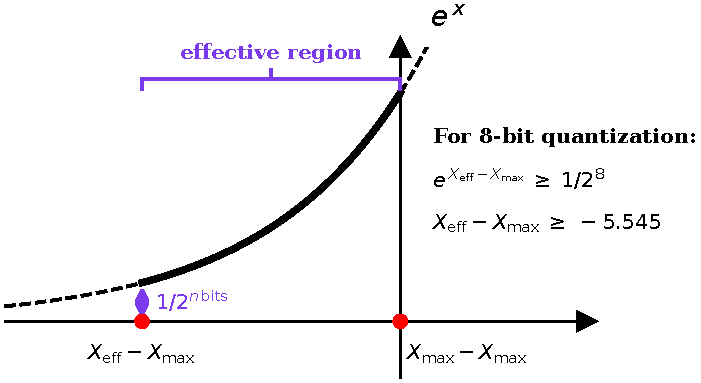
\includegraphics[width=0.75\columnwidth]{figures_analysis/effective_exp.pdf}%
        \label{fig:softmax-eff}}\\[-15pt]
    \subfloat[]{%
        \includegraphics[width=0.8\columnwidth,page=4,trim=1 19 1 1,clip]{figures/TVLSI_drawing.pdf}%
        \label{fig:softmax-unit}}
    \caption{Softmax module. (a)~Effective range of $\exp(\cdot)$ on the shifted argument $X_{i}{-}X_{\max}$ that justifies the six-entry exponential LUT. (b)~Softmax compute unit.}
    \label{fig:softmax}
\end{figure}

The PPE is split into two stages, as shown in Fig.~\ref{fig:arch}. PPE1 is paired with each RMMPE and quantizes the accumulated result back to 8-bit before it leaves the local datapath; PPE2 is shared by all $P$ chains and hosts the non-linear pipeline. After a tile completes, the output rows shift from Accumulator Memory into PPE1. The left bias path inside PPE1 covers the direct (with or without bias adding), ReLU, and layer normalization modes through a shared bias adder and quantizer, with the quantization scale selected per-row. The right softmax-truncator path discerns the large values of $X_{i}{-}X_{\max}$ and forces small ones to zero before forwarding to PPE2. PPE2 then applies ReLU or softmax to the stream, or passes it through unchanged.

The PPE accepts inputs from the $P$~RMMPEs in sequential order, and every mode processes $M$ output rows in parallel.

\subsubsection{Direct and ReLU Mode}
\label{sec:arch-ppe-direct}

The direct mode is enabled by bypassing the bias adder in PPE1 and selecting the direct path in PPE2. Substituting ReLU for the direct path checks the sign bit of the incoming sample, emitting zero when the MSB is~$1$ and the original value when the MSB is~$0$; the cost is a single comparator per PE column.

\subsubsection{Layer Normalization Mode}
\label{sec:arch-ppe-ln}

The layer normalization mode executes the RFN computations: the precomputed running statistics fold into the per-row quantization scale of the existing bias-and-quantize path, so the on-chip operation reduces to a sequence of multiplies and adds, with no dedicated normalization datapath. If the original layer normalization formulation is needed instead, the output matrix can be exported to an external mean-and-standard-deviation unit, after which the fused scale is written back into the RMMPE and a second drain of Accumulator Memory completes the standard LN computation.

\subsubsection{Softmax Mode}
\label{sec:arch-ppe-softmax}

The softmax mode realizes the log-sum-exp form as a fixed-point dataflow that requires two drains of Accumulator Memory and two drains of Softmax Memory:
\begin{equation}
    \mathrm{softmax}(\mathbf{X_i}) = \exp\!\Big(X_{i} - X_{\max} - \ln\!\sum_{j=1}^{K} e^{X_{j} - X_{\max}}\Big)
    \label{eq:softmax}
\end{equation}
The on-die pipeline is shown in Fig.~\ref{fig:softmax}(b), which is color-coded into five stages: \textbf{diff} (red), \textbf{sum} (yellow), \textbf{ln} (purple), \textbf{minus} (blue), and \textbf{exp} (green). Softmax Memory is $1,024$ entries deep and $3$ bits wide, which is sized to hold one full attention row of up to $1,024$ tokens. For longer token sequences, FlashAttention~\cite{Dao2022flashattention} style softmax tiling scheme can be adopted to recover the full sequence softmax score from tiled partial softmax scores off-die.

\emph{First Accumulator Memory drain.} The first drain of Accumulator Memory reduces the multiplier-bank partial sums through the per-row adder tree and pushes the resulting $X_i$ values into PPE1's max register, yielding $X_{\max,\ell}$, the maximum of the $128$ elements held in the current Accumulator Memory row. This drain is bookkeeping only and is not drawn in Fig.~\ref{fig:softmax}(b).

\emph{Second Accumulator Memory drain (diff).} The second drain re-streams the reduced $X_i$ values into the red \textbf{diff} block in Fig.~\ref{fig:softmax}(b). The block forms $X_{\max,\ell} - X_i$ and applies the threshold comparator: any value larger than $6$ would round $\exp(X_i - X_{\max})$ to zero under the 8-bit quantization budget (Fig.~\ref{fig:softmax}(a)) and is clipped before the Softmax Memory write, while the surviving values lie in $[0, 6]$ and fit in the $3$-bit-wide Softmax Memory cell. The \textbf{diff} stage simultaneously records this segment's $X_{\max,\ell}$ into a small per-segment register file. Since one Accumulator Memory row holds $128$ entries, an attention row of length $L > 128$ is processed in $L/128$ %such 
(first drain $\rightarrow$ diff) phases. Each phase producing $128$ shifted entries in the next Softmax Memory segment and one entry in the per-segment register file. Once the entire row has been written, the row-level maximum is recovered from this register file by a final max-reduction, and a per-segment offset $\delta_{\ell}$ is derived for each segment:
\begin{align}
    X_{\max}      &= \max_{\ell}\, X_{\max,\ell}, \label{eq:softmax-xmax}\\
    \delta_{\ell} &= X_{\max} - X_{\max,\ell}. \label{eq:softmax-delta}
\end{align}
Here $\delta_{\ell} \ge 0$ is the constant that the downstream \emph{sum} and \emph{minus} stages add to every Softmax Memory entry from segment $\ell$ to shift its locally-referenced argument $X_{\max,\ell}{-}X_i$ into the globally-referenced argument $X_{\max}{-}X_i$.

\emph{First Softmax Memory drain (sum and ln).} Once the whole row has been written to Softmax Memory and $X_{\max}$ has been resolved across segments, Softmax Memory is drained into the yellow \textbf{sum} block. Each entry indexes the six-element exponential LUT that stores $e^{-1},\dots,e^{-6}$, exactly the bins that cover the effective region of Fig.~\ref{fig:softmax}(a). After the per-segment offset $\delta_{\ell}$ is added so that the LUT argument is $X_i - X_{\max}$ in the global reference frame. The LUT output enters an adder that accumulates the global denominator $\Sigma = \sum_i \exp(X_i - X_{\max})$ in a single register shown at the top right of Fig.~\ref{fig:softmax}(b).

Once \emph{sum} completes, the purple \textbf{ln} block computes $\ln \Sigma$ by the approximation of~\cite{meiqi2018softmax}:
\begin{equation}
\begin{aligned}
    \Sigma      &= 2^{w} \cdot k, \qquad k \in [1, 2), \\
    \ln \Sigma  &= \ln 2 \cdot \log_{2} \Sigma = \ln 2 \cdot (w + \log_{2} k) \\
                &\approx \ln 2 \cdot (w + k - 1).
\end{aligned}
\label{eq:loge}
\end{equation}
Since $k \in [1, 2)$, the last line applies the Mitchell approximation $\log_{2} k \approx k - 1$ on $[1, 2)$. In hardware, a leading-one detector (LOD) extracts $w$; a $-1$ adder folds the mantissa $k$ to $k{-}1$, which is then multiplied by $\ln 2$ to produce the natural logarithm.

\emph{Second Softmax Memory drain (minus and exp).} The second Softmax Memory drain re-streams the stored differences. For each entry $i$, the blue \textbf{minus} block forms the full argument of the outermost exponential in Eq.~\eqref{eq:softmax}, $X_i - X_{\max} - \ln \Sigma$, by subtracting $\ln \Sigma$ from the Softmax Memory value (after the per-segment offset $\delta_{\ell}$). The green \textbf{exp} block then evaluates
\begin{equation}
    e^{x} = 2^{x \log_{2} e} = 2^{i+d} = 2^{i} \cdot 2^{d} = 2^{d} \gg -i,
    \label{eq:exp}
\end{equation}
where $x \le 0$ and $(i, d)$ are the integer and fractional parts of $x \log_{2} e$: a small $2^{d}$ LUT indexed by $d$ and a shift by $-i$ produce $\mathrm{softmax}(\mathbf{X_i})$~\cite{meiqi2018softmax}.

\emph{Scheduling.} The two Accumulator Memory drains run in sequence, and Accumulator Memory cannot %free to 
receive the next matmul's partial sums until the second drain finishes. The two Softmax Memory drains, by contrast, do not touch Accumulator Memory, so they overlap with the next matmul's computing latency. Softmax mode therefore exposes one extra Accumulator Memory drain per attention segment relative to other modes, with the remainder of the pipeline downstream of Softmax Memory hidden behind the next matrix multiply. With the above design, no iterative function units are required.

\subsection{Discussion on Addressing Challenges}
\label{sec:arch-challenges}

We close this section by mapping the four challenges of Section~\ref{sec:intro} to the hardware constructs described above.

\subsubsection{Scalability}
\label{sec:arch-challenges-scalability}

The RMMPE exposes the three configurable design parameters $N$, $M$, and $P$ introduced above. The three knobs are independent, so the same architecture re-targets across the model-size envelope without datapath redesign.

\subsubsection{Flexibility}
\label{sec:arch-challenges-flexibility}

The transformer model is partitioned into a sequence of (GEMM, PPE-path) pairs. Every pair maps onto the accelerator without further reconfiguration because all input and weight matrices share the RRLC format, and the output materializes in row-wise order, so only a small row buffer is required rather than a full output matrix. Multiple RMMPEs in the chain share the same weight stream during a tile pass, so the reuse exposed by the row-wise schedule is fully exploited.

An additional opportunity, untapped in the single-chip prototype, is the parallelism that opens up across attention heads and across the FFN GEMMs. During the multi-head attention stage, the heads are independent and can execute on independent accelerator instances; during the FFN stage, each instance produces a subset of the output rows. Because layer normalization is row-wise and the activation function is element-wise, the per-instance row subsets proceed through their local PPEs without cross-instance communication, so a multi-chip extension does not require an interconnect for the non-linear path.

\subsubsection{Sparsity-Compatibility}
\label{sec:arch-challenges-sparsity}

Sparsity awareness reduces both external-memory traffic and on-chip cycles: the multiplications between zero weights and their corresponding activation elements are skipped, and the RRLC \textit{Run} pointer drives the address generator so that zero MACs never enter the multiplier array. The pattern is element-wise unstructured, so the algorithm side retains full freedom over which weights to drop.

\subsubsection{Non-Linearity}
\label{sec:arch-challenges-nonlinearity}

The PPE approximates every non-linear function with multiplications, additions, and shifts: the softmax LUT and leading-one-detect logarithm, the RFN fusion, and the single-comparator ReLU. The chip executes the residual non-linear path without leaving the on-die fabric, at the accuracy budget reported in Table~\ref{tab:accuracy}.

% =========================================================================
% \section{Top-Level Scheduling}
% \label{sec:sched}

% The four operating modes of the accelerator---direct GEMM, no-bias GEMM, softmax, and layer normalization-fused GEMM---share a single load--stream--drain template: an activation tile is written into Input Memory, a weight tile is streamed through the PE chain consuming the activation, and Accumulator Memory is drained through the appropriate post-PE branch. Only the post-PE configuration and, in the softmax mode, an additional drain over Softmax Memory distinguish one mode from another. The four cases are illustrated in Fig.~\ref{fig:sched}.

% \begin{figure}[!t]
%     \centering
%     \framebox[\columnwidth]{\rule{0pt}{6cm}\TODO{Fig.~\ref{fig:sched}: four-panel top-level scheduling figure --- to be drawn by user per \texttt{src/figures-todo/fig-top-scheduling.md}. Panels show, for each of the four operating modes (direct, no-bias, softmax, layer-norm), the tile shapes (activation, weight, and output), the schedule timeline, and the active post-PE branch.}}
%     \caption{Top-level scheduling of the four supported transformer operating modes. Each mode reuses the same load--stream--drain cycle; only the post-PE branch and, in the softmax case, a second drain of Accumulator Memory differ. \TODO{User caption once figure is drawn.}}
%     \label{fig:sched}
% \end{figure}

% The scheduler interface is small. At the start of each weight tile, the address generator inside every RMMPE is reset; at the end of MAC, an accumulator-drain command shifts the accumulated partial sums from Accumulator Memory into PPE1; in the softmax mode only, a second drain command later shifts Softmax Memory into PPE2. Three tile-completion flags mark the end of one tile pair, the end of one weight tile (one column-group of the output), and the end of one activation tile (one row-group of the output). Outer iteration over multiple weight or activation tiles uses no additional control: a fresh address-generator reset simply restarts the inner loop on the next tile.

% The softmax mode is the only mode whose schedule departs from the load--stream--drain template, because the baseline two-pass softmax requires Accumulator Memory to be drained twice: once to extract $X_{\max}$ and once to compute $X_{i}{-}X_{\max}$. Section~\ref{sec:arch-lsoft} eliminates the second pass via a tile-fused running-max / log-sum-exp recurrence, simplifying the scheduler back to one drain even for softmax.

% =========================================================================

\begin{figure}[!t]
    \centering
    \includegraphics[width=\columnwidth,page=5,trim=1 1 1 1,clip]{figures/TVLSI_drawing.pdf}
    \vspace{-27pt}
    \caption{Annotated die micrograph of the 28\,nm prototype.}
    \label{fig:die}
\end{figure}

\begin{figure}[!t]
    \centering
    \includegraphics[width=0.9\columnwidth,page=6,trim=1 1 1 1,clip]{figures/TVLSI_drawing.pdf}
    \vspace{-10pt}
    \caption{Silicon measurement setup.}
    \vspace{-10pt}
    \label{fig:setup}
\end{figure}

\section{Silicon Implementation and Results}
\label{sec:results}

We prototyped the propsoed sparse transformer accelerator in TSMC~28\,nm CMOS, which employs the~$8{\times}8{\times}8$ configuration for $N{\times}M{\times}P$. This section reports the measured silicon characterization, the per-model sparsity impact on speedup, on-chip energy, weight external memory access (EMA), the on-chip non-linear-function linearization gain, the flexibility/scalability comparison against a 2D systolic array baseline, and a comparison with prior transformer accelerators.

\subsection{Die Micrograph and Measurement}
\label{sec:results-die}

% Generated from src/spec.xlsx; style modeled on src/summary.png (grid lines
% with shaded left column for parameter names).
\begin{table}[!t]
    \caption{Measured silicon summary.}
    \label{tab:summary}
    \centering
    \footnotesize
    \setlength{\tabcolsep}{3pt}
    \renewcommand{\arraystretch}{1.25}
    \begin{tabular}{%
        |>{\columncolor[gray]{0.92}\centering\arraybackslash}m{0.44\columnwidth}%
        |>{\centering\arraybackslash}m{0.40\columnwidth}|}
        \hline
        \rowcolor[gray]{0.80}
         & \textbf{Chip Summary} \\
        \hline
        \textbf{Technology} & TSMC 28\,nm \\ \hline
        \textbf{Die area} & 9.26\,mm$^2$ \\ \hline
        \textbf{On-chip SRAM} & 317\,KB \\ \hline
        \textbf{PE config. ($N{\times}M{\times}P$)} & $8{\times}8{\times}8$ \\ \hline
        \textbf{Supply voltage} & 0.75\,--\,1.10\,V \\ \hline
        \textbf{Frequency} & 24\,--\,400\,MHz \\ \hline
        \textbf{Precision} & INT8 \\ \hline
        \textbf{Power} & 12.7\,--\,244.2\,mW \\ \hline
        \textbf{Peak performance$^{1,2}$} & 1.634\,TOPS \\ \hline
         & ViT-Base$^{4}$: 20.32\,TOPS/W \\ \cline{2-2}
        \multirow{-2}{=}{\centering\textbf{Energy efficiency$^{2,3}$}}
            & BERT-base$^{5}$: 21.93\,TOPS/W \\ \hline
        \textbf{Area efficiency$^{1,2}$} & 0.176\,TOPS/mm$^2$ \\ \hline
    \end{tabular}\\[2pt]
    {\scriptsize $^{1}$\,at 1.10\,V, 400\,MHz; $^{2}$\,90\,\% model sparsity; $^{3}$\,at 0.77\,V, 183\,MHz; \\ $^{4}$\,ImageNet-1K; $^{5}$\,GLUE benchmark.}
\end{table}


\begin{figure}[!t]
    \centering
    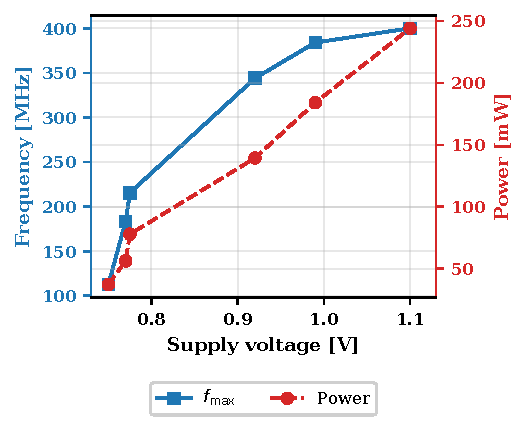
\includegraphics[width=\columnwidth]{figures_analysis/vf_scaling.pdf}
    \vspace{-20pt}
    \caption{Measured peak frequency (left axis, blue) and total chip power (right axis, red) versus logic supply voltage over the prototype's supply-scaled operating points.}
    \vspace{-15pt}
    \label{fig:vf}
\end{figure}

Fig.~\ref{fig:die} shows the annotated die micrograph of the 28\,nm prototype. The eight RMMPE tiles, each paired with its PPE1, are placed around the global weight memory in a ring that supports the cascaded weight streaming bus. The prototype chip occupies a $9.26$\,mm$^{2}$ area in TSMC 28\,nm CMOS, with $317$\,KB of on-chip SRAM.

Fig.~\ref{fig:setup} shows the measurement setup. The chip is mounted on a test PCB and driven by a host FPGA that handles I/O streaming and control logic. The FPGA in turn is configured from a host PC that issues the test vectors and reads back the inference output. A power supply provides the power, an oscilloscope probes the on-die signals brought out to the pad ring, and an energy analyzer (Joulescope) measures voltage and current.

Under this setup we characterize the chip at nine operating points across the~$0.75$\,--\,$1.10$\,V logic-supply range. Table~\ref{tab:summary} reports the headline numbers, and Fig.~\ref{fig:vf} plots peak frequency (left axis) and total chip power (right axis) versus logic supply at the six supply-scaled points. Peak frequency rises from~$112.6$\,MHz at $0.75$\,V to~$400$\,MHz at $1.10$\,V, while total power scales from~$37.2$\,mW to~$244.2$\,mW over the same voltage range. The full~$24$\,--\,$400$\,MHz envelope in Table~\ref{tab:summary} extends below~$112.6$\,MHz by sharing the~$0.75$\,V floor, useful for low-throughput inference. At the $1.10$\,V, $400$\,MHz peak-performance corner, the chip delivers $1.634$\,TOPS on a $90\,\%$-sparse workload, giving an area efficiency of $0.176$\,TOPS/mm$^{2}$. At the peak-efficiency operating point of $0.77$\,V, $183$\,MHz, the same $90\,\%$ sparsity yields $20.32$\,TOPS/W on ViT-Base (ImageNet-1K) and $21.93$\,TOPS/W on BERT-base (GLUE).

\subsection{Sparsity}
\label{sec:results-sparsity}

The chip's sparsity-aware datapath demonstrates two related benefits: it preserves accuracy at high pruning ratios because the RRLC format imposes no structural constraint on the mask, and it converts that accuracy headroom into measurable on-chip speedup because every zero MAC is skipped at zero cycle cost. %This subsection quantifies both halves in three figures.

\subsubsection{Compute Reduction vs Accuracy}
\label{sec:results-sparsity-acc}

\begin{figure}[!t]
    \centering
    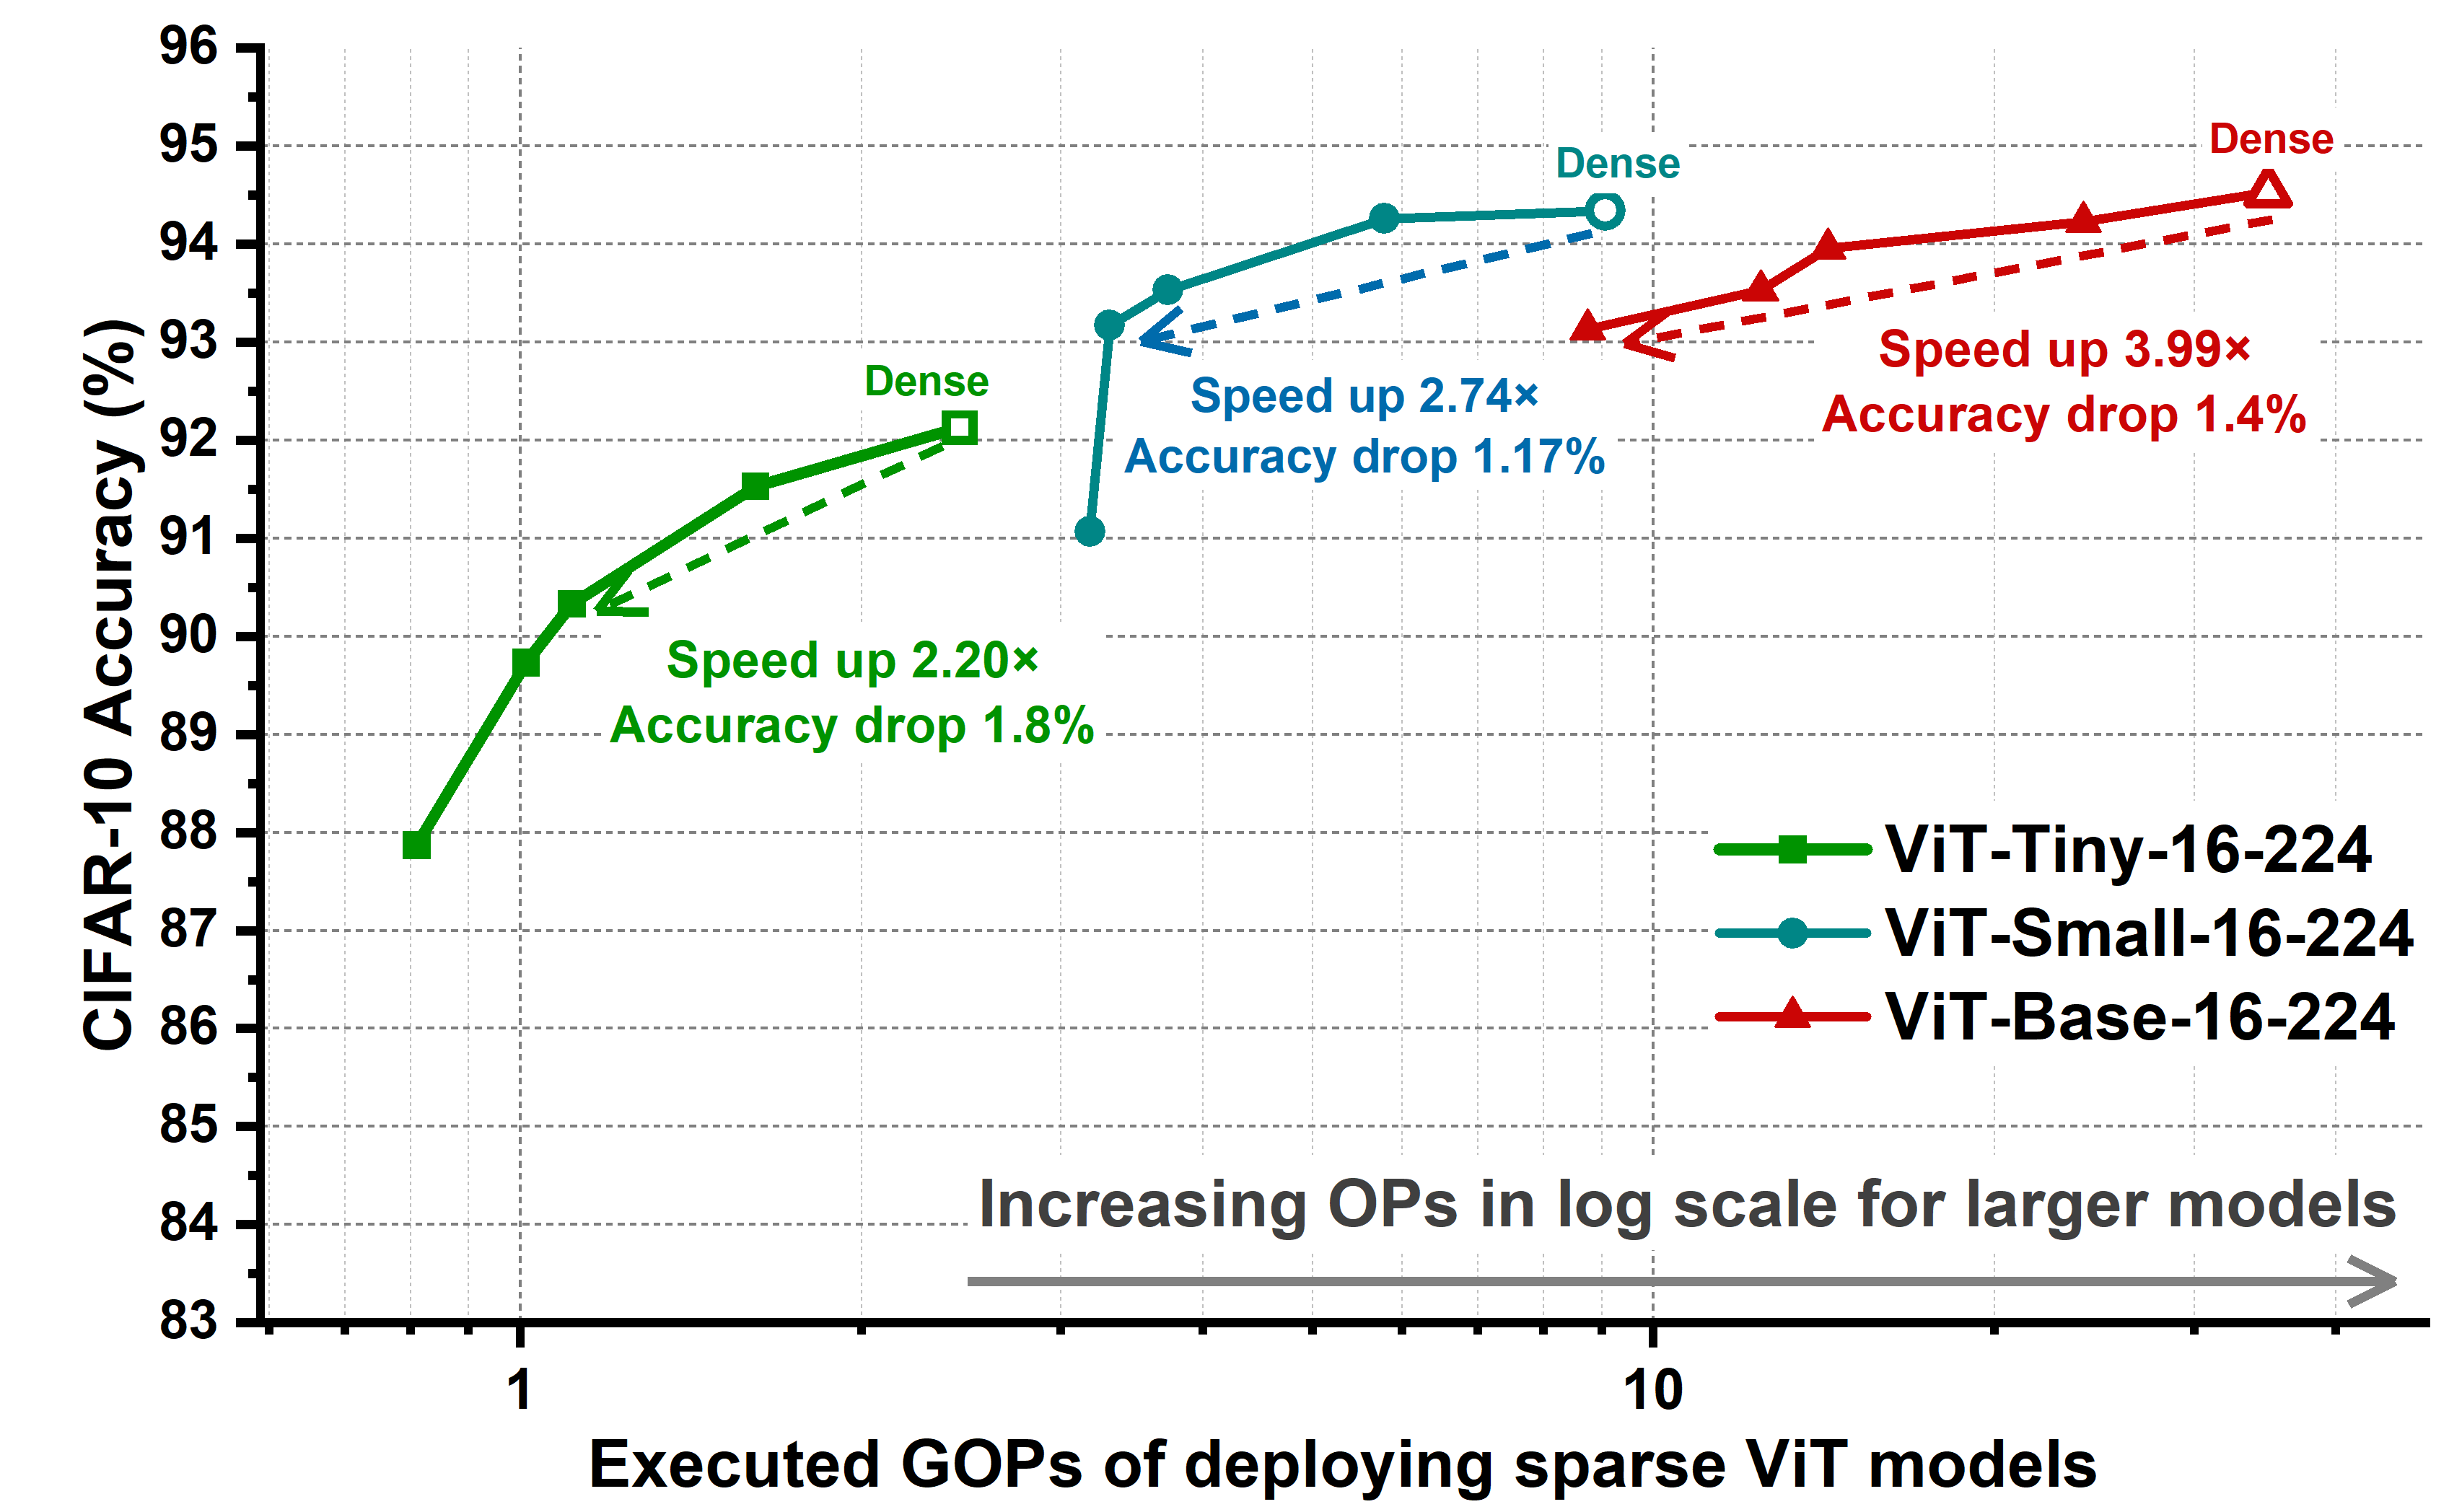
\includegraphics[width=\columnwidth]{figures/FLOPs_vs_Accuracy.png}
    \vspace{-20pt}
    \caption{Model accuracy versus executed non-zero operations on CIFAR-10 for ViT-Tiny, ViT-Small, and ViT-Base across the sparsity sweep at sparsity levels of $0\%$, $50\%$, $75\%$, $80\%$, and $90\%$.}
    \vspace{-10pt}
    \label{fig:flops-acc}
\end{figure}

Fig.~\ref{fig:flops-acc} plots model accuracy against the number of executed non-zero operations across the per-model sparsity sweep. The task is single-image CIFAR-10 classification. The accuracy drop is sub-percentage point through $80\%$ sparsity for the larger two models. At~$80\%$ sparsity, ViT-Base loses~$1.0$\% %,pp 
and ViT-Small loses~$1.17$\% accuracy. %,pp. 
At~$90\%$ sparsity the gap stays at $1.4$\% %,pp 
for ViT-Base. ViT-Tiny, with its smaller redundancy budget, reaches a $1.8$\% %,pp 
accuracy drop already at $75\%$ sparsity and is the model with the steepest accuracy decline. At each model's best practical sparse operating point, the executed GOPs reduce by $2.20\times$ for ViT-Tiny at $75\%$ sparsity, $2.74\times$ for ViT-Small at $80\%$ sparsity, and $3.99\times$ for ViT-Base.

\subsubsection{Speedup and Energy across Sparse Models}
\label{sec:results-sparsity-energy}
A furthur evaluation of the sparisty impact on the on-chip execution of ViT-Small, ViT-Base, and BERT-base is shown in Fig.~\ref{fig:sparsity-energy}. The four bars for each model correspond to the dense baseline and the four sparsity ratios of $60\%$, $70\%$, $80\%$, and $90\%$. ImageNet-1K classification is the task for the ViT models, and a $128$-token GLUE-style input is the task for BERT-base. 
%The three subplots show (a)~the whole-model FLOPs-reduction speedup, (b)~the per-inference on-chip energy at the peak-performance operating point, and (c)~the RRLC-compressed weight EMA per inference.

\begin{figure}[!t]
    \centering
    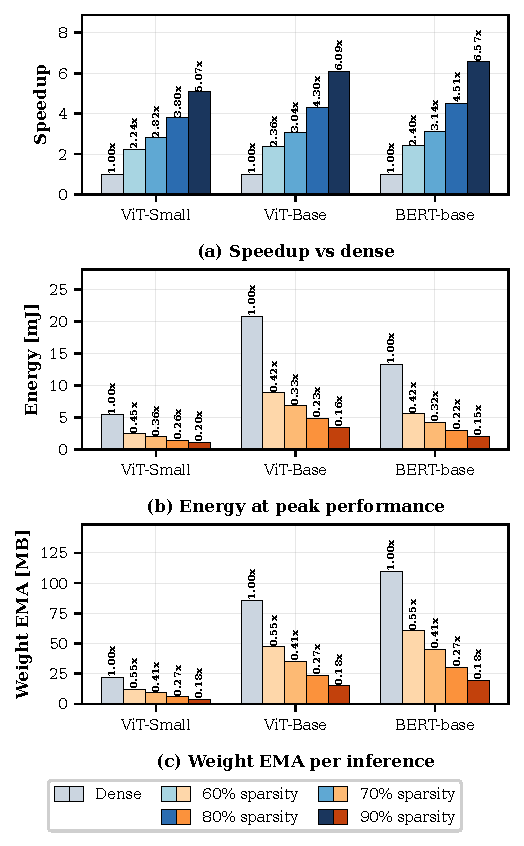
\includegraphics[width=\columnwidth]{figures_analysis/sparsity_energy_latency.pdf}
    \caption{Sparsity impact on ViT-Small, ViT-Base, and BERT-base at the dense baseline and the four sparsity ratios. (a)~Whole-model FLOPs-reduction speedup. (b)~Per-inference on-chip energy at the peak-performance operating point. (c)~RRLC-compressed weight EMA per inference. Inference is batch-1 ImageNet-1K for the ViT models and a $128$-token GLUE-style input for BERT-base.}
    \label{fig:sparsity-energy}
\end{figure}

Fig.~\ref{fig:sparsity-energy}(a) shows that the overall model speedup rises monotonically with sparsity for every model, reaching $5.07\times$ on ViT-Small, $6.09\times$ on ViT-Base, and $6.57\times$ on BERT-base at $90\%$ sparsity. The speedup is highest for the model with the largest sparsifiable (FFN) FLOPs fraction, because the attention matrix multiplications $Q\!\cdot\!K^{\top}$ and $A\!\cdot\!V$ have no weight matrix and pass through unsparsified, forming a fixed floor that caps the attainable speedup. ViT-Small carries $7.9\%$ of its per-block FLOPs in those unsparsified operations (the smaller hidden dimension $H{=}384$ leaves less compute in the four weighted GEMMs), versus $4.1\%$ for ViT-Base and only $2.7\%$ for BERT-base whose shorter sequence shrinks the attention contribution. Consequently, As shown in Fig.~\ref{fig:sparsity-energy}(a), the speedup is highest for BERT-base, followed by ViT-Base and ViT-Small models.
%the speedup orders BERT-base, ViT-Base, and ViT-Small in Fig.~\ref{fig:sparsity-energy}(a). 
Above $87.5\%$ sparsity, the mean gap between non-zeros ($=s/(1{-}s)$) %first 
exceeds the 3-bit \textit{Run} cap of $7$, and the encoder must insert placeholder \textit{Run}${=}7$ tuples to bridge longer runs. The padding factor (tuples consumed per real non-zero) reaches $9/7 \approx 1.29\times$ at $90\%$ sparsity, which divides the ideal sparsity saving by $1.29$ and clips the FLOPs reduction by $1 - 1/1.29 \approx 22\%$ on the weighted ops. The absolute speedup at $90\%$ sparsity still grows monotonically from the $80\%$ bar, but falls roughly a factor of two short of the ideal $1/(1{-}s) = 10\times$ that a padding-free encoding would deliver.

Fig.~\ref{fig:sparsity-energy}(b) translates the compute-reduction trend into per-inference on-chip energy. Each sparse bar is annotated with its ratio to the dense baseline, which equals the inverse of the speedup because compute time and the $P_{\text{total}}{\times}t$ energy product scale linearly with the compressed-FLOPs count. At $90\%$ sparsity, the energy drops to $0.20\times$ for ViT-Small, $0.16\times$ for ViT-Base, and $0.15\times$ for BERT-base, i.e., a $5{-}7\times$ energy reduction relative to dense execution on the same chip. The dense-normalized ratios on top of the sparse bars are invariant to the chosen operating point: the absolute energies at the peak-efficiency operating point are about half of those shown here, but the per-model ratios are unchanged.

Fig.~\ref{fig:sparsity-energy}(c) shows the RRLC-compressed weight EMA per inference. Under the $8$-bit \textit{Value} plus $3$-bit \textit{Run} encoding ($11$ bits per non-zero), the compressed weight footprint falls from the INT8 dense baseline of $22$, $86$, and $110$\,MB for ViT-Small, ViT-Base, and BERT-base to $6.05$, $23.65$, and $30.25$\,MB at $80\%$ sparsity ($3.6\times$ smaller), and to $3.89$, $15.20$, and $19.45$\,MB at $90\%$ sparsity ($5.7\times$ smaller). The marginal saving from $80\%$ to $90\%$ is smaller than from $60\%$ to $80\%$ because of the same RRLC padding factor that clips the speedup curve in Fig.~\ref{fig:sparsity-energy}(a).

\subsubsection{Unstructured vs.~Structured Sparsity}
\label{sec:results-sparsity-struct}

Many prior sparse-transformer accelerators support only structured sparsity patterns: NVIDIA Ampere and Hopper tensor cores restrict the weight layout to the $2{:}4$ pattern~\cite{nvidia2020structuredsparsity}, and recent academic designs further fix the granularity to $1{:}4$ or coarse-grained block sparsity to amortize the indexing hardware~\cite{Hanrui2021SpAtten,Hubara2021AcceleratedSparse, Eunji2023TF-MVP}. The PLATON pruning study reports that, at the same target sparsity, unstructured pruning consistently preserves higher model accuracy than the corresponding structured layout~\cite{zhang2022platon}, because the unstructured mask can drop the least-important weight wherever it lies rather than the $(M{-}N)$-th-smallest weight in every group of $M$. The accelerator presented here supports unstructured sparsity natively through the RRLC \textit{Run} pointer, and the same pointer collapses any N:M layout into a degenerate case of the row-wise schedule at identical compute density. The architecture therefore admits the higher-accuracy unstructured pattern at any sparsity level while still accommodating structured sparsity for workloads or toolchains that prefer the constrained form.

\subsection{Non-Linear Function Linearization}
\label{sec:results-nonlinear}

The hardware-aware reformulations fold the residual non-linear operations into hardware-friendly forms: softmax is approximated with a six-entry exponential LUT and a leading-one-detect logarithm; layer normalization is fused into the per-row quantization scale via running feature normalization; and GELU is replaced by ReLU as the FFN activation. Fig.~\ref{fig:nonlinear-lin} quantifies the cumulative latency saved at each of these three steps on one transformer block of ViT-Base and BERT-base, assuming both the baseline and the chip provision $P{=}8$ parallel non-linear function lanes.

\begin{figure}[!t]
    \centering
    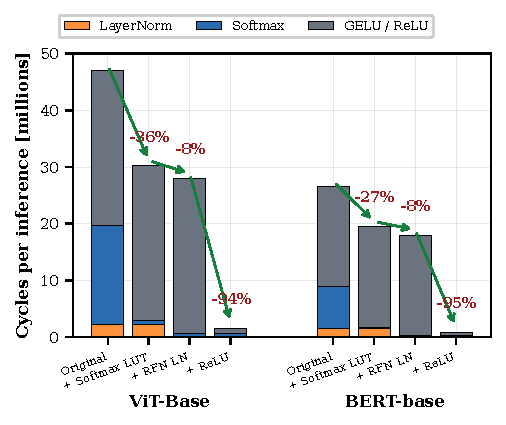
\includegraphics[width=\columnwidth]{figures_analysis/nonlinear_linearization.pdf}
    \vspace{-20pt}
    \caption{Cumulative latency reduction from the three non-linear linearization steps on a single transformer block. Bars are stacked by operator.}
    \vspace{-10pt}
    \label{fig:nonlinear-lin}
\end{figure}

Three observations are noteworthy. First, the softmax LUT shrinks the softmax segment from the dominant slice of the original bar to a thin sliver, reducing the per-inference non-linear latency by $36\%$ for ViT-Base and $27\%$ for BERT-base in a single step; the difference between models is attributable to the larger attention-element count in ViT-Base's longer sequence. Second, RFN contributes a more modest $8\%$ reduction because layer normalization operates on fewer elements than softmax or GELU; nevertheless, RFN eliminates the layer normalization segment entirely and is fused with quantization path. Third, replacing GELU with ReLU collapses the largest remaining segment by approximately $30\times$ per element, yielding the biggest single reduction in the chain ($94\%$\,--\,$95\%$). Cumulatively across the three steps, the per-inference non-linear cycle cost drops from $46.97$\,M to $1.61$\,M for ViT-Base and from $26.54$\,M to $0.88$\,M for BERT-base, a $97\%$ reduction at the same SFU count for both models. The model-independent shape of the reduction, where softmax LUT and ReLU substitution both yield order-of-magnitude per-element savings, indicates that the linearization choices generalize across any transformer block built from these three primitives.

\subsection{Flexibility and Scalability}
\label{sec:results-flex-scale}

The RMMPE imposes a \emph{one-dimensional} alignment constraint on the workload: in the chosen mode, only a single workload axis (input rows for row-wise, weight columns for column-wise) needs to be a multiple of the spatial tile $M{\cdot}P$ for the multiplier array to operate at $100\%$ utilization. The inner-K ($K_{\text{para}}$) parallelism number $N$ (the contraction-dimension multiplications performed per cycle, introduced in Section~\ref{sec:arch-rmmpe}) imposes a separate constraint that the GEMM's inner dimension $K$ be a multiple of $N$; this is almost always satisfied for ViT-Base's hidden dimension $H{=}768$, FFN intermediate $F{=}3072$, and head dimension $d{=}64$. A two-dimensional systolic array of shape $S_r{\times}S_c$ instead enforces both axes simultaneously. This subsection quantifies the throughput consequence on the six operators of one ViT-Base transformer block (QKV, output projection $O$, FFN1, FFN2, $QK^{\top}$, $AV$); for the two batched-attention BMMs the per-head batch dimension is flattened into the row count so that $M{=}n_{\text{heads}}{\cdot}L$, with the token sequence length $L{=}197$ and $n_{\text{heads}}{=}12$.

\begin{figure}[!t]
    \centering
    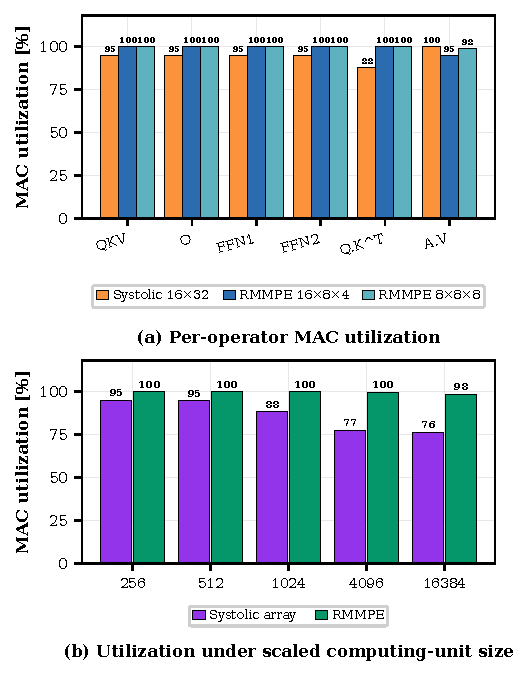
\includegraphics[width=\columnwidth]{figures_analysis/flexibility_scalability.pdf}
    \vspace{-20pt}
    \caption{Flexibility and scalability against a square systolic array baseline on ViT-Base. (a)~Per-operator MAC utilization at $512$ multipliers. (b)~Workload-FLOPs-weighted utilization at five matched multiplier budgets.}
    \vspace{-10pt}
    \label{fig:flex-scale}
\end{figure}

\subsubsection{Per-operator flexibility} Fig.~\ref{fig:flex-scale}(a) compares three $512$-multiplier configurations at the operator level: a $16{\times}32$ rectangular systolic array (2D-constrained baseline); an RMMPE shaped $N{=}16$, $M{=}8$, $P{=}4$ (tile $M{\cdot}P{=}32$, $K_{\text{para}}{=}16$), chosen to share the systolic array's $16{\times}32$ outer shape for a fair-multiplier-budget comparison; and the prototype's own $8{\times}8{\times}8$ configuration (tile $M{\cdot}P{=}64$, $K_{\text{para}}{=}8$). In the two RMMPE configurations the numbers play different roles than they do for the systolic array: only the spatial tile $32$ (or $64$) is an output-axis constraint, while the second number is the inner-K constraint that all ViT-Base inner dimensions $\{H, F, d\}$ satisfy. The matched-budget RMMPE reaches $100\%$ on five of the six operators and $94.7\%$ on $AV$ where the inner-K constraint $K{=}L{=}197$ does not divide $N{=}16$; the chip's $8{\times}8{\times}8$ configuration relaxes the inner-K to $N{=}8$ and lifts $AV$ to $98.5\%$ at no cost on the other operators. The $16{\times}32$ systolic array, by contrast, pays its $16$-row tax on every operator with $M{=}L{=}197$ (pinning the four linear GEMMs at $94.7\%$) and an additional $32$-column tax on $QK^{\top}$ ($87.8\%$).

\begin{table*}[!t]
    \caption{Comparison with prior sparse transformer accelerators.}
    \label{tab:comparison}
    \centering
    \footnotesize
    \setlength{\tabcolsep}{4pt}
    \renewcommand{\arraystretch}{1.25}
    \begin{tabular}{%
        |>{\columncolor[gray]{0.92}\centering\arraybackslash}m{1.4in}%
        |>{\centering\arraybackslash}m{0.85in}%
        |>{\centering\arraybackslash}m{0.85in}%
        |>{\centering\arraybackslash}m{0.85in}%
        |>{\centering\arraybackslash}m{0.85in}%
        |>{\columncolor[gray]{0.96}\centering\arraybackslash}m{0.95in}|}
        \hline
        \rowcolor[gray]{0.80}
            & \textbf{ISSCC'22\,\cite{Yang2022isscc}}
            & \textbf{ISSCC'23\,\cite{Thierry2023isscc}}
            & \textbf{CICC'25\,\cite{Li2025SparseTrim}}
            & \textbf{VLSI'25\,\cite{Fan2025MultiTaskTransformer}}
            & \textbf{This work} \\ \hline
        \textbf{Technology (nm)}                 & 28              & 12               & 28               & 22                 & 28 \\ \hline
        \textbf{Area (mm$^{2}$)}                 & 6.82            & 4.60             & 0.667            & 5.80               & 9.26 \\ \hline
        \textbf{Supply voltage (V)}              & 0.56\,--\,1.10  & 0.62\,--\,1.00   & 0.35\,--\,0.90   & 0.55\,--\,0.90     & 0.75\,--\,1.10 \\ \hline
        \textbf{Frequency (MHz)}                 & 50\,--\,510     & 77\,--\,717      & 6.55\,--\,262    & 75\,--\,400        & 24\,--\,400 \\ \hline
        \textbf{SRAM (KB)}                       & 336             & 647              & 45.7             & 576                & 317 \\ \hline
        \textbf{Data precision}                  & INT12           & FP4/FP8          & INT8             & INT4/INT8          & INT8 \\ \hline
        \textbf{Sparsity support}                & Unstructured    & Unstructured     & Unstructured     & Block-wise struct. & Unstructured \\ \hline
        \textbf{Non-linear support}              & yes             & yes              & no               & yes                & yes \\ \hline
        \textbf{Power (mW)}                      & 12.06\,--\,272.8 & 10\,--\,122     & 0.43\,--\,54     & 19.6\,--\,197.1    & 12.7\,--\,244.2 \\ \hline
        \textbf{Peak perf. (TOPS)}               & 0.52\,--\,4.07$^{1}$ & 0.367\,(FP8) & --               & 0.92\,(INT8)$^{3}$ & 1.634$^{4}$ \\ \hline
        \textbf{Peak energy eff. (TOPS/W)}       & 1.91\,--\,27.56$^{1}$ & 8.24\,(FP8)$^{2}$ & 9.49\,--\,51.8$^{1}$ & 12.52\,(INT8)$^{3}$ & 20.32\,--\,21.93$^{4}$ \\ \hline
        \textbf{Peak area eff. (TOPS/mm$^{2}$)}  & 4.04            & 0.0798           & --               & 0.159              & 0.176 \\ \hline
    \end{tabular}\\[2pt]
    {\scriptsize $^{1}$\,matmul with 90\,\% sparsity on both input and weight;\quad $^{2}$\,matmul with 50\,\% input sparsity; \\ \quad $^{3}$\,matmul with 87.5\,\% weight sparsity; \quad $^{4}$\,model average with 90\,\% weight sparsity.}
    \vspace{-15pt}
\end{table*}

\subsubsection{Scalability} Fig.~\ref{fig:flex-scale}(b) sweeps the multiplier budget from $256$ to $16{,}384$ at matched configurations. At each budget the first dimension of the systolic array ($S_r$) and the first dimension of the RMMPE ($N$) are held equal to a common value $S$, and the remaining axes ($S_c$ for the systolic array, $M{\cdot}P$ for the RMMPE) are sized to fill the same total multiplier count; this keeps the two designs on equal footing and isolates the effect of the 2D vs.~1D alignment constraint. The RMMPE recovers the spatial mismatch that costs the systolic array increasingly more multipliers as $S$ grows: at $S{=}16$ ($256$ muls) the systolic array loses about $5$\,pp on the $M{=}L{=}197$ axis, and the gap widens to $+11.6$\,pp at $1024$ multipliers (systolic array $32{\times}32$ rounds both axes against $L{=}197$, RMMPE applies the $32$ only where it fits) and $+22.1$\,pp at $4096$ multipliers ($64{\times}64$ systolic array crosses $L{=}197$ and incurs the row-tile boundary on the four GEMMs simultaneously, while the RMMPE uses column-wise to align the $64$ with the $H$, $F$ axes that are multiples of $64$). At $16{,}384$ multipliers, the matched RMMPE has $N{=}128$, and the inner-K constraint $K{=}d{=}64{<}N$ now costs $50\%$ on $QK^{\top}$; nevertheless the workload-weighted utilization remains $98\%$ versus the systolic array's $76\%$, because $QK^{\top}$ accounts for only $2\%$ of the per-block FLOPs.

The architecture-level constraint reduction translates directly into measured throughput. The systolic array baseline must pay for two simultaneous alignments per operator and runs out of headroom on ViT-Base at $1,024$ multipliers; the RMMPE pays for one, picks the favorable axis per operator via mode selection, and only begins to see a comparable tax at $16{,}384$ multipliers and then only on the operator whose inner dimension is smaller than the multiplier-budget-driven $K_{\text{para}}$. A further asymmetry favors the RMMPE on sparse workloads: row-wise mode accelerates compute by skipping zero-weight multiplications via the RRLC \textit{Run} pointer, and column-wise mode (with weights stationary) cannot skip the multiplications with zeros in weight, but still benefits from the compressed weight EMA off-chip and from activation sparsity aware frameworks~\cite{Tang2024QUEST}. A 2D systolic array gains no advantage from either form of sparsity. The flexibility/scalability advantage therefore compounds with the sparsity benefit at every multiplier budget studied here, with the gap widest at the largest budgets.

\subsection{Comparison with State-of-the-Art Accelerators}
\label{sec:results-comp}

Table~\ref{tab:comparison} compares our chip against four recent transformer accelerators~\cite{Yang2022isscc, Thierry2023isscc, Li2025SparseTrim, Fan2025MultiTaskTransformer}.
%accelerator~1 (ISSCC'22~\cite{Yang2022isscc}), accelerator~2 (ISSCC'23~\cite{Thierry2023isscc}), accelerator~3 (CICC'25~\cite{Li2025SparseTrim}), and accelerator~4 (VLSI'25~\cite{Fan2025MultiTaskTransformer}). 
This chip supports arbitrary unstructured sparsity together with an on-die linearized non-linear pipeline, the combination needed to execute a full transformer end-to-end on the same fabric. Against \cite{Thierry2023isscc} and \cite{Fan2025MultiTaskTransformer}, %accelerators~2 and~4, 
our chip is better on all three headline metrics: peak performance ($1.634$\,TOPS vs.~$0.367$ and $0.92$\,TOPS), peak energy efficiency ($20.32$\,--\,$21.93$\,TOPS/W vs.~$8.24$ and $12.52$\,TOPS/W), and peak area efficiency ($0.176$ vs $0.0798$ and $0.159$\,TOPS/mm$^{2}$). 
This chip's energy efficiency is $1.62\times$\,--\,$2.47\times$ higher than \cite{Thierry2023isscc, Fan2025MultiTaskTransformer}. 
%accelerators~2 and~4. 
Both \cite{Yang2022isscc} and \cite{Li2025SparseTrim} %Accelerators~1 and~3  
report their headline metrics (up to $4.07$\,TOPS, $51.8$\,TOPS/W, and $4.04$\,TOPS/mm$^{2}$) at a matmul-pair operating point with $90\%$ sparsity on \emph{both} weight and activation, an isolated peak that not every matmul inside a transformer block can hit. In particular, the attention BMMs $QK^{\top}$ and $AV$ carry no weight sparsity at all. Our results reported here are model-averaged values, instead of peak sparse-matmul values.

% =========================================================================
\section{Conclusion}
\label{sec:conclusion}

This paper presented a 28\,nm sparse transformer accelerator that addresses the four design challenges of transformer-targeted hardware: scalability, flexibility, sparsity-compatibility, and on-chip non-linearity. Our chip applies row-wise matrix multiplication on a row-wise run-length-coded operand stream to handle the heterogeneous matrix shapes and to accelerate unstructured sparsity. The %extendedly supported 
column-wise matrix multiplication further improves the flexibility and efficiency for model deployment. It linearizes softmax, layer normalization and other non-linear functions. Measured silicon achieves~$20.32$\,TOPS/W on ViT-Base and~$21.93$\,TOPS/W on BERT-base at~$90\,\%$ sparsity at the peak-efficiency operating point. This chip is $1.62$--$2.47\times$ better in energy efficiency compared to other sparse transformer accelerators at same sparsity configuration and level. Our chip demonstrates that arbitrary unstructured sparsity and the residual non-linearities of transformer inference can both be handled inside a single sparse-matmul fabric without resorting to off-chip arithmetic or structurally restricted sparsity patterns.

% Render URLs/DOIs in the bibliography as plain monospace text (no clickable
% hyperlink). \cite{} links in the body of the paper remain clickable.
\renewcommand{\url}[1]{\nolinkurl{#1}}
\bibliographystyle{IEEEtran}
\bibliography{reference}

\vfill

\end{document}
